\documentclass[a4paper,11pt]{article}
\usepackage{geometry}
%%If you need more control on the margins and other options:
%\usepackage[left=2.5cm,right=2.5cm,top=2.5cm,bottom=2.5cm,twoside]{geometry}
%% The amssymb package provides various useful mathematical symbols
\usepackage{amssymb}
%% The amsthm package provides extended theorem environments
\usepackage{amsthm}
%% The amsmath package facilitates writing math formulas and improves the typographical quality of their output
\usepackage{amsmath}
%% The tikz package allows you to draw nice figures and graphs
\usepackage{tikz}
\usetikzlibrary{arrows}
\usetikzlibrary{shapes}
%%The hyperref package allows you to incorporate hyperlinks and URLs
\usepackage{hyperref}

%% You can construct your own commands to use in this document
% \newcommand{\todo}[1]{{\large\bf TODO: }#1\ensuremath{\Box}}
\newcommand\myworries[1]{\textcolor{red}{#1}}

\title{Template - 2015/2016}

\author{NA}
\date{\today} 
%%If you do not want a date to display:
%\date{}


\begin{document}
\maketitle


\begin{abstract}
Here you can write a short abstract of your paper, which will be displayed on the title page.
\end{abstract}

\section{A section}
You can start with a section... This is \LaTeX! \\      % make a latex logo
Or make a space after \LaTeX\ like this! \\
Also try this \TeX

\subsection{A subsection}
In which you can make a subsection...

\subsubsection{A subsubsection}
or even a subsubsection.

\paragraph{A paragraph}
A paragraph can also be made within a section, which will not count in the table of contents.

\section*{Section without numbering}
If you do not like numbered (sub(sub))sections, you can add an asterisk to the command.

\paragraph{Mathematics}
You can type inline equations easily, like $\int_0^\infty 3x^2-x+10$, but you can also enter the math environment:
\[
\int_0^\infty 3x^2-x+10
\]
or you can have multiline equations:
\begin{align}
\max & \sum_{j} u_{j} x_{j} \label{eq:obj}\\
s.t. & \notag \\
&\sum_{j} x_{j} \leq 1 &&\forall j \in \mathcal{J} \label{eq:xonce}\\
&x_{j} \in \{0,1\} &&\forall j \in \mathcal{J} \label{eq:binarydecvar}
\end{align}
and you can reference a particular line in the equation, for example the objective function \eqref{eq:obj}, and you can suppress the numbering for particular lines using \texttt{\textbackslash notag}.

\section{Tables and figures}
Here we can see some nice statistics of two people in Table \ref{table:johnmary} and the \LaTeX logo in Figure \ref{fig:latexlogo}. \\      %line break
We can also use the \texttt{tikz} package to draw figures ourselves, like the graphs in Figures \ref{fig:graph} and \ref{fig:simplegraph}.

\begin{table}[!htpb]
\centering
{\begin{tabular}{|l|c|r|}
\hline
 & John & Mary\\
\hline
Age (years)	& 25   & 23 \\
Height (m)	& 1.80 & 1.62\\
\hline
\end{tabular}}
\caption{Statistics of John and Mary.
\label{table:johnmary}}
\end{table}

\begin{figure}[!htpb]
\centering
{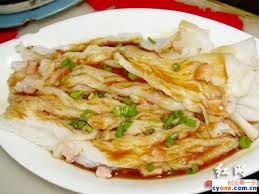
\includegraphics[scale=0.1]{kill_for_this}}
\caption{The logo for \LaTeX.
\label{fig:latexlogo}}
\end{figure}

\begin{figure}[!htpb]
\centering
{\scriptsize
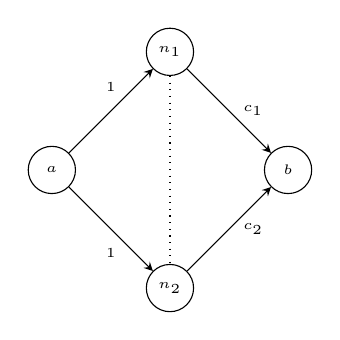
\begin{tikzpicture}[>=stealth, scale=0.75,every node/.style={minimum size=0.6cm, inner sep=0pt, font=\tiny}]
	%Source
	\node [circle,draw] (source) at (0,0) {$a$};
	%Nodes
	\node [circle,draw] (n1) at (2,2) {$n_1$};
	\node [circle,draw] (n2) at (2,-2) {$n_2$};
    \draw[->] (source) edge node [above]{1} (n1);
    \draw[->] (source) edge node [below]{1} (n2);
	\draw[dotted] (n1) edge node {} (n2);
	%Sink
	\node [circle,draw] (sink) at (4,0) {$b$};
	\draw[->] (n1) edge node [right] {$c_1$} (sink);
    \draw[->] (n2) edge node [right] {$c_2$} (sink);
\end{tikzpicture}
}
\caption{A graph network
\label{fig:graph}}
\end{figure}

\begin{figure}[!htpb]
\centering
{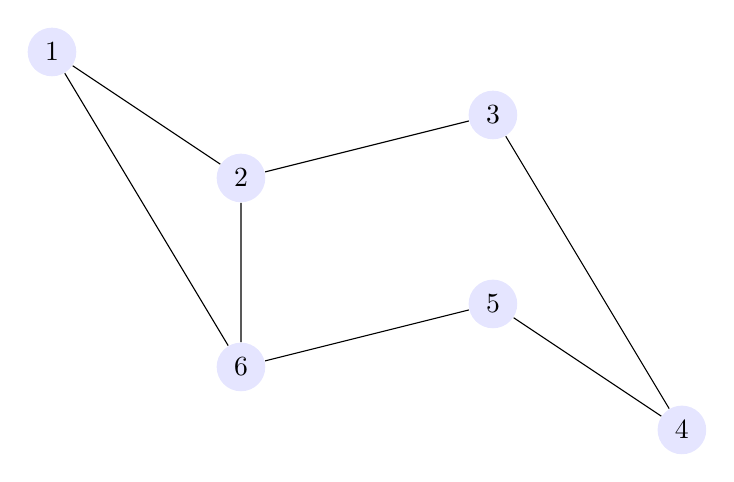
\begin{tikzpicture}
  [scale=.8,auto=left,every node/.style={circle,fill=blue!10}]
  \node (n1) at (1,10) {1};
  \node (n2) at (4,8)  {2};
  \node (n3) at (8,9)  {3};
  \node (n4) at (11,4) {4};
  \node (n5) at (8,6)  {5};
  \node (n6) at (4,5)  {6};

  \foreach \from/\to in {n1/n2,n2/n3,n3/n4,n4/n5,n5/n6,n1/n6,n6/n2}
    \draw (\from) -- (\to);

\end{tikzpicture}
}
\caption{A simple graph.
\label{fig:simplegraph}}
\end{figure}

\paragraph{References}
You can make use of BibTeX or a local bibliography. For the latter, an example can be found below. You can cite references by making use of \texttt{\textbackslash cite}, like \cite{cmoler2004}. With BibTeX you have more options, see also \url{https://en.wikibooks.org/wiki/LaTeX/Bibliography_Management}.

% \todo{Here's something I might need to change.}
\myworries{I'm worried about the text}

%%Page break
\newpage
\begin{thebibliography}{99} 
%%the widest-label parameter (99) has been set assuming less than 100 numbered items in the bibliography
\bibitem{cmoler2004}
  Moler, C.,
  \emph{Numerical Computing with MATLAB},
  Society for Industrial and Applied Mathematics,
  2004.

\end{thebibliography}

\end{document}